
\subsubsection{Exploration Time}
\label{subsubsec:agg-time}

\begin{figure}[h]
\vspace{-8pt}
	\centering
		\subfloat[OpenVX: Diff \#ACCs] {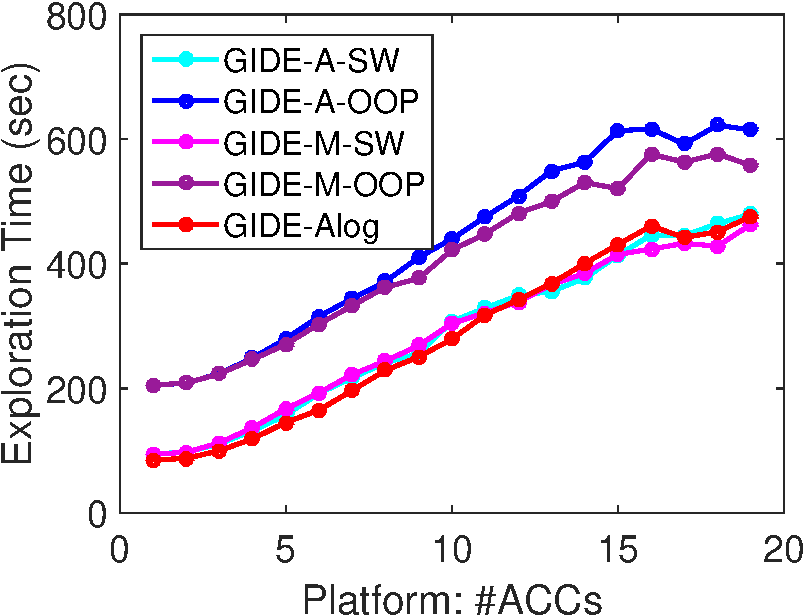
\includegraphics[width=.48\linewidth]{fig/timeACCs.pdf}\label{fig:timeACCs}}
		\hfill
		\subfloat[Synthetic: Diff \#Apps] {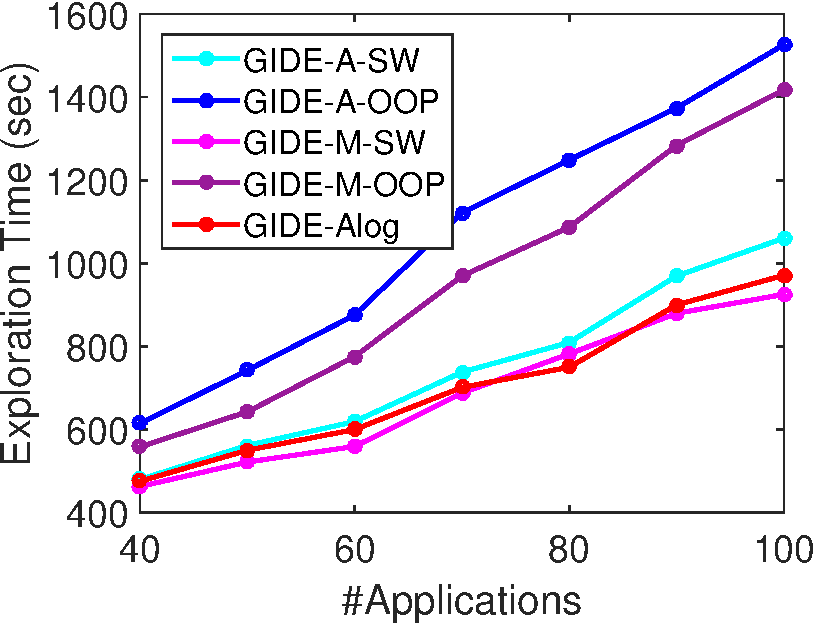
\includegraphics[width=.48\linewidth]{fig/timeApps.pdf}\label{fig:timeApps}}
	\vspace{-8pt}
	\caption{Exploration Time}
	\label{fig:exTime}
\end{figure}

\newtext{
\figref{fig:exTime} shows the exploration time of UPA with different aggregations running on Intel i5-3450 with 3.10GHz. In \figref{fig:timeACCs}, the UPA exploration time increases with the increasing of ACCs budget.  
the $A \mhyphen ODP$ and $M \mhyphen ODP$ are much slower than other aggregations because their normalization needs to find the optimal platform of each application (an exploration problem in itself). In average, the time of finding optimal platforms in $A \mhyphen ODP$ and $M \mhyphen ODP$ takes 32.56\% of total exploration. While, $A \mhyphen SW$, $M \mhyphen SW$ and $Alog$ evaluations do not need these optimal platforms. 
After ACCs>16, DSE exploration time stops increasing, because there are only 35 OpenVX unique kernels in applications, which could be instantiated once in HW. The design complexity of 16-19 ACCs from 35 kernels is not increased significantly.


\figref{fig:timeApps} describes the exploration time with an increasing number of applications, which are synthetically generated.
With the number of applications increasing, the $A \mhyphen ODP$ and $M \mhyphen ODP$ exploration time increase much faster than $A \mhyphen SW$, $M \mhyphen SW$ and $Alog$. The reason is that the number of application optiaml platform search dramatic increases the exploration time of $M \mhyphen ODP$ and $A \mhyphen ODP$. 
}


\begin{table}[h]
	\caption{Comparison of Aggregations in UPA}
	\vspace{-8pt}
	\label{tab:cmp}
	\centering
	\arraybackslash
	\begin{tabular}{>{\centering\arraybackslash}p{0.125\linewidth}|>{\centering\arraybackslash}p{0.25\linewidth}|>{\centering\arraybackslash}p{0.25\linewidth}|>{\centering\arraybackslash}p{0.175\linewidth}}
		\toprule
		& $rEFF_{SW}$ View & $rEFF_{ODP}$ View & Scalability \\
		\midrule
		
		\hline
		A-SW & Bad (low- med- EFF apps) & Bad (low- med- EFF apps) & Good \\
		\hline
		A-OOP & Good & Good & Bad \\
		\hline
		M-SW & Bad (high- EFF apps) & Bad (high- EFF apps) & Good \\
		\hline
		M-OOP & Bad (low- med- EFF apps) & Bad (low- EFF apps) & Bad \\
		\hline
		Alog & Good & Good & Good \\
		
		\bottomrule
	\end{tabular}
\end{table}

\newtext{
\tabref{tab:cmp} summaries the performance of UPA with different aggregations. 
$A \mhyphen SW$ has a good for scalability, however, platform efficiency is bad for low- and median-efficiency applications. 
$A \mhyphen ODP$ platform achieves good efficiency for all applications, but it has bad scalability since its normalization needs to explore the optimal platform for each application. 
Both $M \mhyphen SW$ and $M \mhyphen ODP$ platforms have bad efficiency, because they are only focus on the median-efficiency application in a certain view ($rEFF_{SW}$ or $rEFF_{ODP}$).
We select $Alog$ as aggregation because it is efficient and fair to all applications. Moreover, it eliminates the need to compute the normalization, i.e., finding the optimal platform for each application.
}